\documentclass[a4paper,ngerman,landscape,12pt]{scrartcl}

\usepackage[utf8]{inputenc}

\usepackage[ngerman]{babel}
\usepackage{hyperref}

\usepackage{graphicx}


\usepackage{lmodern}
\usepackage{tabto}
\usepackage{multicol}

\usepackage[normalem]{ulem}

\setlength\parskip{\medskipamount}
\setlength\parindent{0pt}

\usepackage{geometry}
\geometry{tmargin=0.2cm,bmargin=0.0cm,lmargin=0.75cm,rmargin=0.75cm}

\pagestyle{empty}

\begin{document}

\begin{center}
  \Huge
  \textbf{\sf Pizzaseminar in Mathematik}

  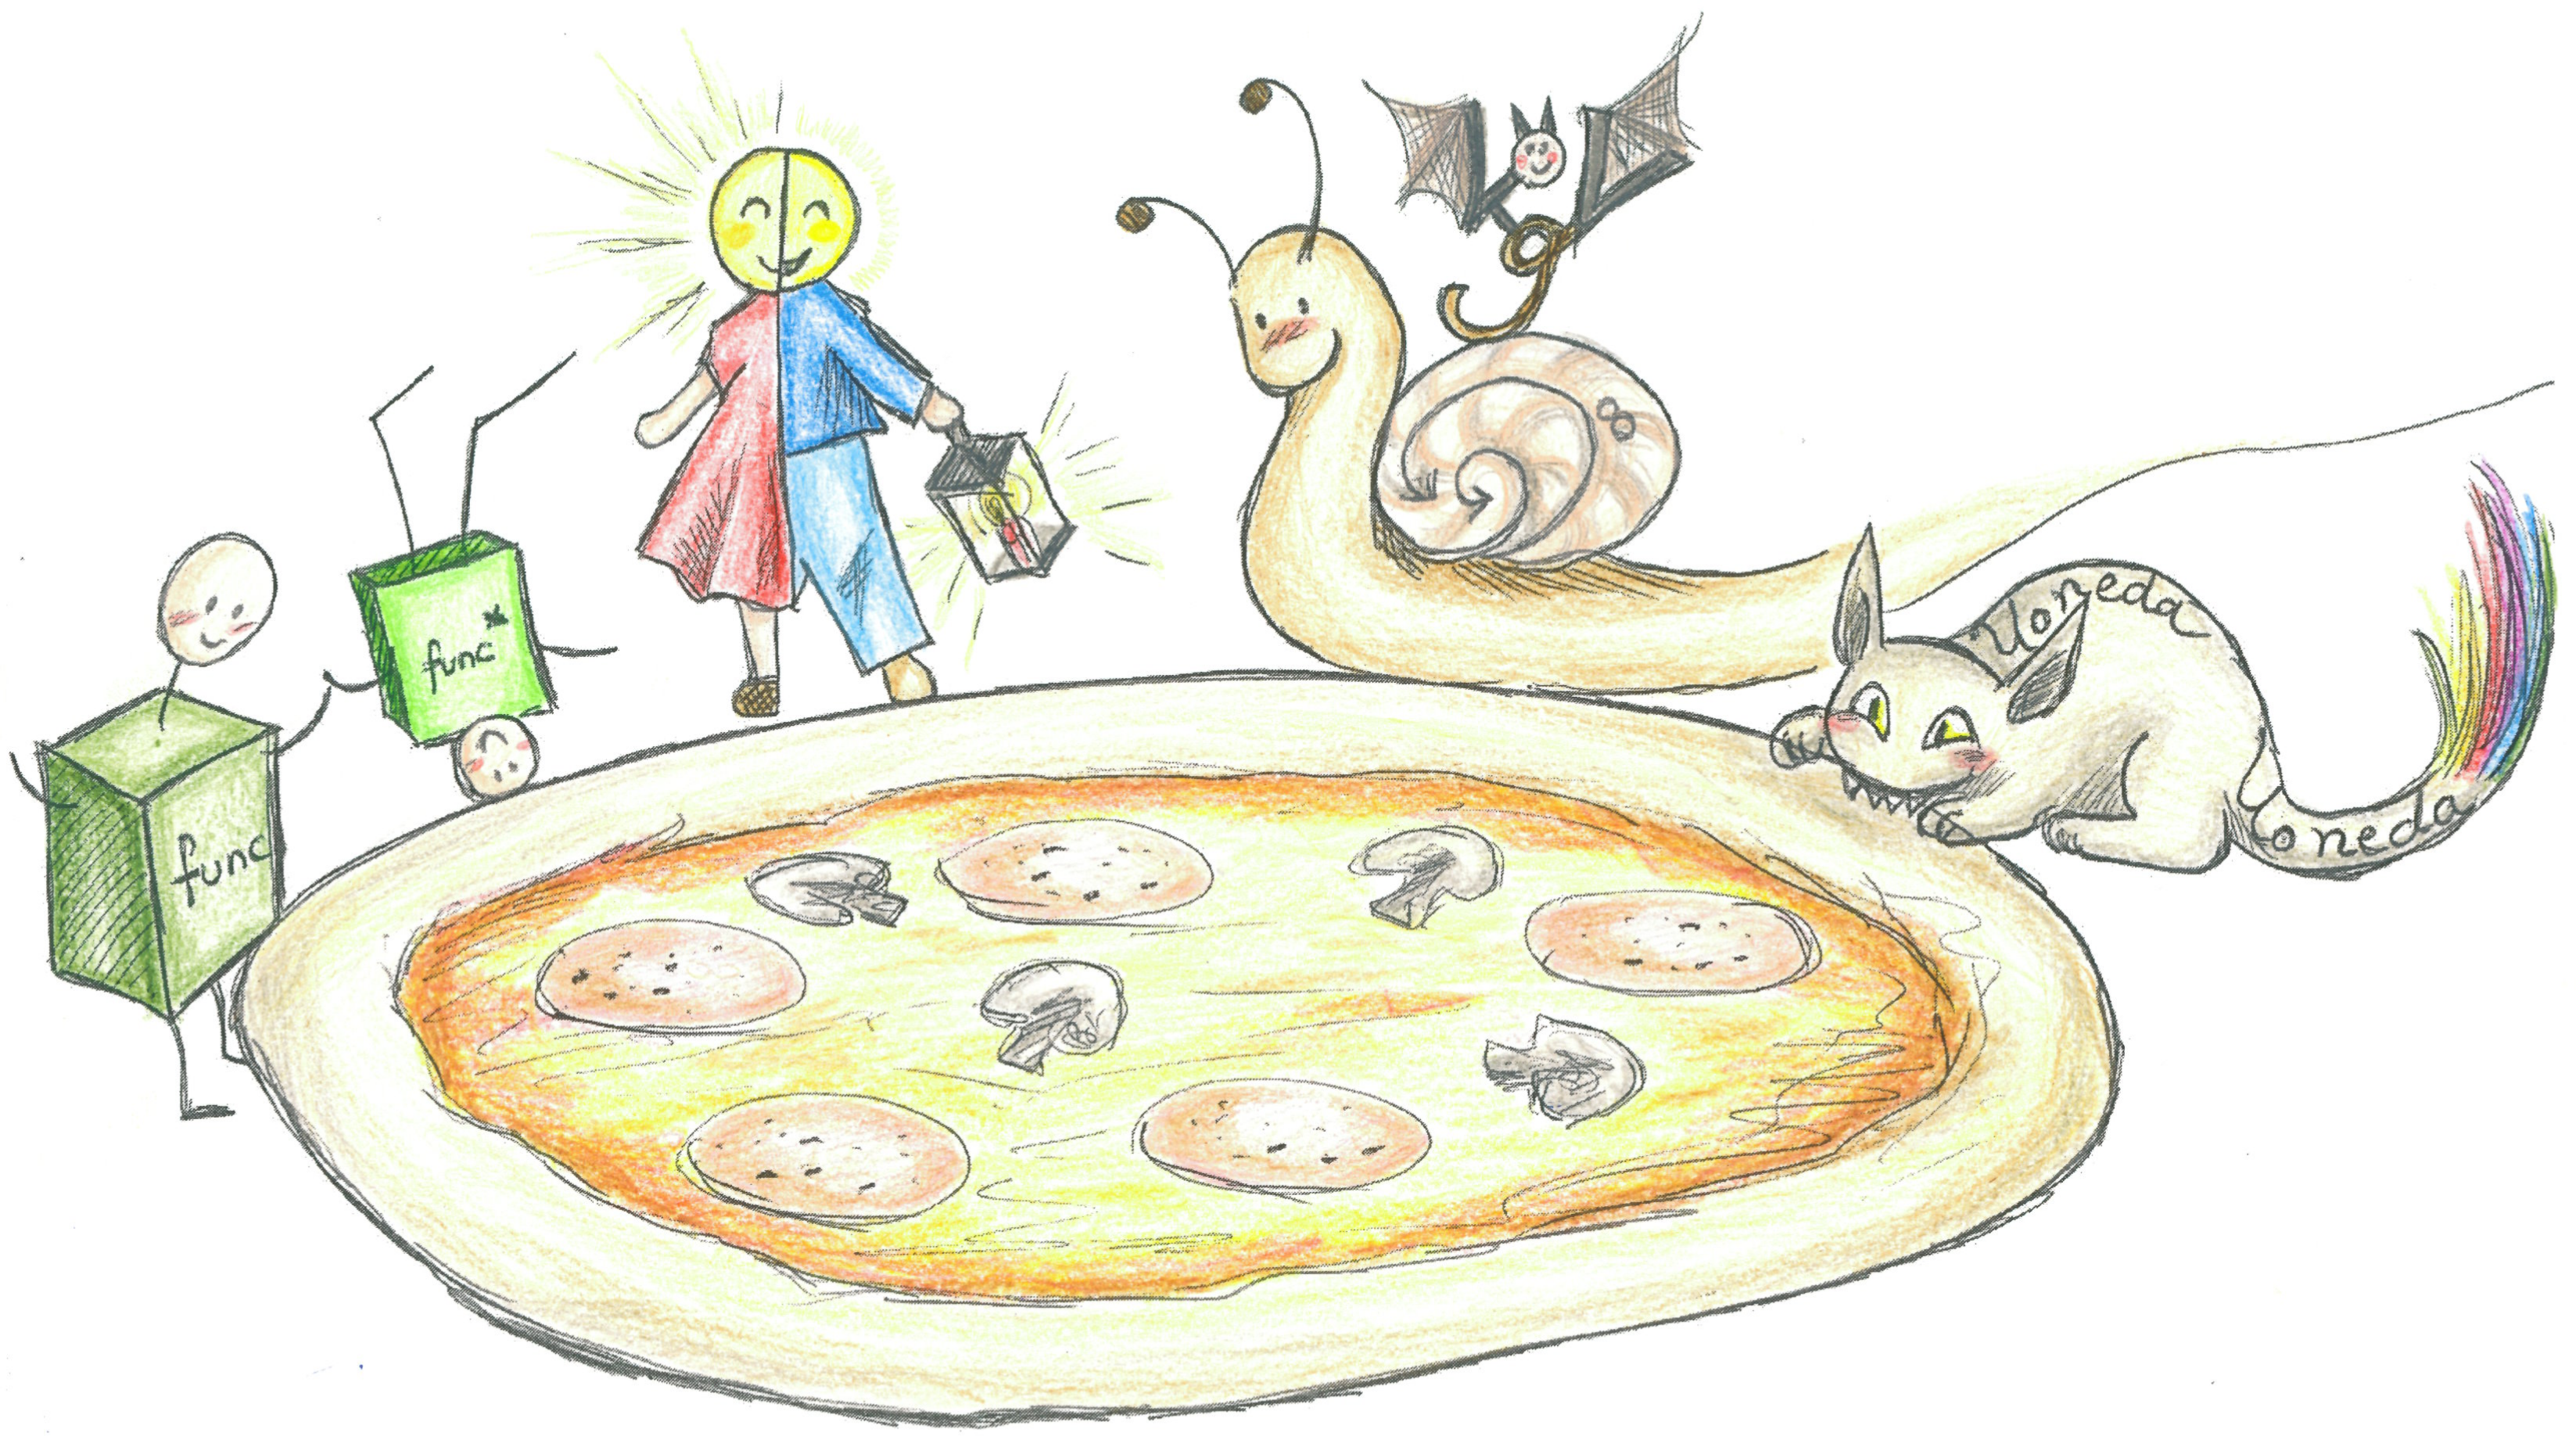
\includegraphics[scale=0.83]{pizza-farbig-hq}

  \vspace{1em}
  \large
  \begin{minipage}{0.95\textwidth}
    \setlength\parskip{\medskipamount}
    \setlength\columnsep{1.5cm}
    \begin{multicols}{2}
\emph{Erzeugende Funktionen sind Wäscheleinen für Folgen.}
Mit ihrer Hilfe kann man komplizierte Formeln auf elegante und kompakte
Weise notieren und manipulieren. Dabei erhalten die vertrauten
Rechenoperationen (Addition, Multiplikation, Differentiation,
\ldots) eine ganz neue Bedeutung.
Erzeugende Funktionen treten an verschiedenen Stellen in
der Mathematik immer wieder auf: Etwa in der Darstellungstheorie, der
algebraischen Topologie, der Stochastik, der Kombinatorik, der
Zahlentheorie und der
Kategorientheorie. Die Theorie der erzeugenden
Funktionen ist elementar
zugänglich, d.\,h. sie setzt kein
fünfjähriges Mathematik-Studium voraus,
wird in einem
fünfjährigen Mathematik-Studium aber
üblicherweise auch nicht behandelt.

Beginn jeweils um 10:30 Uhr in Raum 2004/L1.

Skript und Übungsblätter: \\
\url{http://pizzaseminar.speicherleck.de/}
\end{multicols}
\newpage
  \end{minipage}

  \begin{minipage}{1.00\textwidth}
  \begin{center}
    \Large
    \begin{tabular}{r@{\quad}l@{\quad}l@{\quad}l}
        1. &
        19.2. &
        Sonja Grob &
        Gewöhnliche erzeugende Funktionen \\[0.1em]
        2. &
        19.2. &
        Tung Nhat Tran &
        Exponentiell erzeugende Funktionen \\[0.1em]
        3. &
        19.2. &
        Jessica Mandl &
        Multivariate erzeugende Funktionen \\[0.1em]
        4. &
        19.2. &
        Simon Kapfer &
        Beispiele \\[0.1em]
        5. &
        26.2. &
        Dominik Xaver Hörl &
        Differenzenrechnung \\[0.1em]
        6. &
        26.2. &
        Matthias Hutzler &
        Schattenkalkül \\[0.1em]
        7. &
        26.2. &
        Peter Uebele &
        Formel von Faà di Bruno \\[0.1em]
        8. &
        12.3. &
        Mirjam Fahrion &
        Symmetrische Polynome \\[0.1em]
        9. &
        12.3. &
        Simon Kapfer &
        Formel von Molien und Pólya-Enumeration \\[0.1em]
        10. &
        26.3. &
        Ingo Blechschmidt &
        Erzeugende Funktionen in der Wahrscheinlichkeitstheorie \\[0.1em]
        11. &
        26.3. &
        Sven Prüfer &
        Bonusthema: Enumerative Geometrie \\[0.1em]
        12. &
        2.4. &
        Kathrin Gimmi &
        Bonusthema: Gromov-Hausdorff-Konvergenz \\[0.1em]
        13. &
        2.4. &
        Tim Baumann &
        Bonusthema: Vier-Farben-Satz
    \end{tabular}

    \includegraphics[scale=0.8]{../erzeugende-funktion}
  \end{center}
  \end{minipage}
\end{center}

% Inhalte/inhaltlich

\end{document}
